\textbf{Encja \textit(entity)} to obiekt przechowywany w bazie. Zbiorem encji nazywamy zbiór obiektów posiadającyh te same atrybuty.
Atrybuty encji mogą być:
\begin{itemize}
    \item proste (o niepodzielnych wartościach) lub złożone (np. adres)
    \item jednoartościowe (np. id) lub wielowartościowe (np. adresy mailowe danej osoby)
    \item pochodne, czyli takie, których wartość oblicza się za pomocą pewnej funkcji na wartościach innych atrybutów
\end{itemize}
Instancje encji są parami różne, więc dla zbioru encji pojęcia superklucza, klucza, klucza głównego i klucza wtórnego działają analogicznie jak
w modelu relacyjnym.
\textbf{Słaba encja} to taka encja, której występuje tylko w kontekście innych encji (np. instytut w kontekście wydziału). Słabe encje nie posiadają własnego identyfikatora, a ich klucz główny zależy również od klucza encji, przy których występują.

\textbf{Związek \textit(relationship)} to wzajemna zależność pomiędzy dwiema lub więcej encjami. Instancja związku reprezentuje związek między instancjami encji.
Związek może być:
\begin{itemize}
    \item unarny, binarny, ternarny, n-arny (klasyfikacja ze względu na stopień)
    \item opcjonalny, obowiązkowy (klasyfikacja ze względu na klasę przynaleźności)
    \item 1 : 1, 1 : M, M : N (klasyfikacja ze względu na typ asocjacyjny)
\end{itemize}
Superkluczem dla \( \mathcal{R} \) zbioru związków o atrybutach \( A_1, \dots, A_k \) pomiędzy zbiorami encji \( E_1, \dots, E_n \) o kluczach głównych \( \text{PK}(E_1), \dots, text{PK}(E_n) \)
jest \( \text{PK}(E_1) \cup \ldots \cup \text{PK}(E_n) \cup \{A_1, \dots, A_k\} \).

\subsection*{Reprezentacja na diagramie}
Do reprezentacji modelu związków encji często wykorzystuje się notację kurzej stopki.

\begin{figure}[h!]
    \centering
    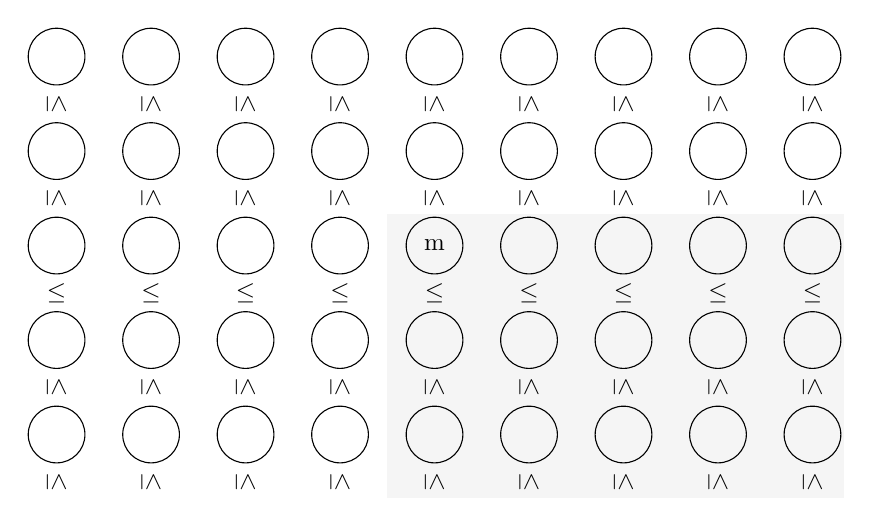
\begin{tikzpicture}[scale=1, every node/.style={scale=0.9}]
  \def\rows{5}
  \def\cols{9}
  \def\cellsize{1.2}

  \filldraw[fill=gray!30, opacity=0.25, draw=none]
    (5*\cellsize - 0.6, -3*\cellsize + 0.4) rectangle
    (9*\cellsize + 0.4, -6*\cellsize + 0.4);

  \foreach \i in {1,...,\rows} {
    \foreach \j in {1,...,\cols} {
      \pgfmathsetmacro\x{\j*\cellsize}
      \pgfmathsetmacro\y{-\i*\cellsize}
      \node[circle, draw, minimum size=8mm] (c\i\j) at (\x,\y) {};
      \ifnum\i=3
        \ifnum\j=5
          \node at (\x,\y) {m};
        \fi
        \node at (\x,\y - 0.6) {\( \leq \)};
      \else
        \node at (\x,\y - 0.6) [rotate=-90]  {\( \leq \)};
      \fi
    }
  }
\end{tikzpicture}
    \caption{Strzałki modelu ER w notacji kurzej stopki}
\end{figure}